\documentclass[12pt]{article}
% \usepackage{polski}
% \usepackage{xcolor}
% \usepackage{pdfcomment}
% \def\PLdateending{\space r.}

\title{L\\
Słownik Lindego t. II s. 578}
\author{Piotr Skowroński (red.)}

\date{\today}

%%%%%%%%%%%%%%%%%%%%%%%%%%%%%%%%%%%%%%%%%%%%%%%%%%%%%%%

\usepackage{fontspec}
\usepackage{xcolor}

%\setmainfont{TeXGyreTermes}
%\setsansfont{TeXGyreTermes}
%\setmainfont{TeXGyreTermes}
%\setmainfont{DejaVu Serif}
%\setmainfont{Bitstream Vera Serif}

% double oblique hyphen:
\setmainfont{Linux Libertine O}
%\setmainfont{Courier New}

%\setmonofont{TeXGyreCursor}
\setmonofont{DejaVu Sans Mono}

% no math
\catcode`\&=12



\usepackage{graphicx}

\usepackage{hyperref}

\usepackage[para]{footmisc}

%%%%%%%%%%%%%%%%%%%%%%%%%%%%%%%%%%%%%%%%%%%%%%%%%%%%%%%

% LaTeX Companion 2nd ed., p. 127
\newcommand{\marginlabel}[1]{\mbox{}\marginpar{\raggedright\hspace{0pt}#1}}

%%%%%%%%%%%%%%%%%%%%%%%%%%%%%%%%%%%%%%%%%%%%%%%%%%%%%%%

\newcommand{\abbrev}[2]{#2}

\newcommand{\entry}[2]{#2}
\newcommand{\entryref}[2]{#2}



% double oblique hyphen
\newcommand{\doh}[1]{⸗}

% http://unifraktur.sourceforge.net/
% UnifrakturMaguntia
\newcommand{\fraktur}[1]{#1}

\newcommand{\gram}[1]{#1}

\newcommand{\mainentry}[2]{#2}
% 1 klasyfikacja hasła
% 2 
\newcommand{\mainentrybegin}[2]{\section{#2}}
% #1 prefiks lub jego brak
% #2 oryginalna pisownia hasła wersalikami
\newcommand{\mainentryend}[1]{}
% #1 oryginalna pisownia hasła wersalikami (powtórzona dla redundacji)
% komenda kończy wcięcie tekstu hasła

\newcommand{\mainentrypageend}[1]{}
% kontynuacja hasła na następnej stronie

\newcommand{\pos}[2]{#2}

\newcommand{\showimage}[1]{\includegraphics[width=1.0\textwidth]{img/#1}}

\newcommand{\quoteref}[1]{#1}

\newcommand{\subentry}[2]{#2}

\newcommand{\wikiq}[2]{\textit{#2}}


\begin{document}
\maketitle

\obeylines



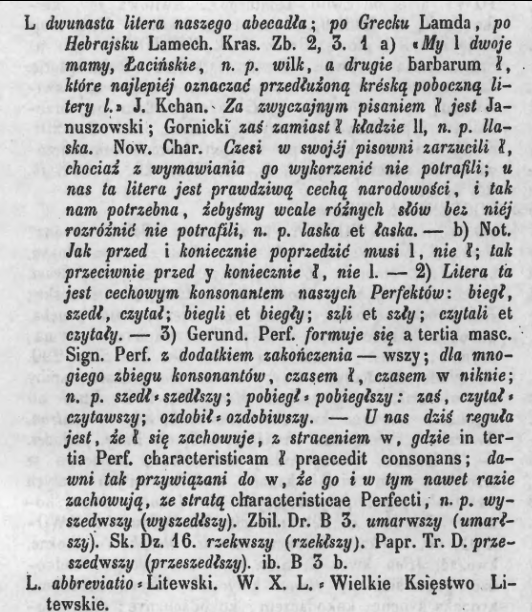
\includegraphics{lindeL.png}

\bigskip
\url{http://teksty.klf.uw.edu.pl/26/3/LindeIIGP+2i.djvu?djvuopts=&page=578&zoom=143&showposition=0.48,0.47}


\newpage

\begin{description}
\item L \textit{dwunasta litera naszego abecadła}; \textit{po Grecku} {\color{yellow} Lamda}, \textit{po Hebrajsku} {\color{blue} Lamech}. Kras. Zb. 2, 3. 1\footnote{Ignacy Krasicki z Zabaw Przyjemnych i Pożytecznych}

a) «\textit{My} l \textit{dwoje  mamy, Łacińskie, n. p. wilk, a drugie barbarum} ł, \textit{które najlepiej oznaczać przedłużoną kréską poboczną litery} l.» J. Kchan.\footnote{Jan Kochanowski}
\textit{Za zwyczajnym pisaniem} ł \textit{jest} Januszowski; 
Gornicki \textit{zaś zamiast} ł \textit{kładzie} ll, \textit{n. p. llaska}. Now. Char.\footnote{Nowy Charakter Polski} 
\textit{Czesi w swojéj pisowni zarzucili} ł, \textit{chociaż z wymawiania go wykorzenić nie potrafili}; \textit{u nas ta litera jest prawdziwą cechą narodowości, i tak nam potrzebna, żebyśmy wcale różnych słów bez niéj rozróżnić nie potrafili, n. p. laska} \textcolor{red}{et} \textit{łaska}. 

b) Not. \textit{Jak przed} i \textit{koniecznie poprzedzić musi} l, \textit{nie} ł; \textit{tak przeciwnie przed} y \textit{koniecznie} ł, \textit{nie} l. 

\item 2) \textit{Litera ta jest cechowym konsonantem naszych Perfektów}: 
\textit{biegł, szedł, czytał; biegli} \textcolor{red}{et} \textit{biegly}; 
\textit{szli} \textcolor{red}{et} \textit{szły}; \textit{czytali} \textcolor{red}{et} \textit{czytaly}.  
 
\item 3) {\color {red} Gerund. Perf.} \textit{formuje się \textcolor{red}{a tertia masc.}} 
\textcolor{red}{Sign. Perf.} \textit{z dodatkiem zakończenia} — wszy; \textit{dla mnogiego zbiegu konsonantów, czasem} ł, \textit{czasem} w \textit{niknie}; 
\textit{n. p. szedł} ⸗ \textit{szedłszy}; \textit{pobiegła} ⸗ \textit{pobiegłszy: zaś, czytał} ⸗ \textit{czytawszy}; \textit{ozdobił} ⸗ \textit{ozdobiwszy}. 
— \textit{U nas dziś reguła jest, że} ł \textit{się zachowuje, z straceniem} w, \textit{gdzie} \textcolor{red}{in tertia Perf. characteristicam} ł \textcolor{red}{praecedit consonans}; \textit{dawni tak przywiązani do} w, \textit{że go i w tym nawet razie zachowują, ze stratą} \textcolor{red}{characteristicae Perfecti}, \textit{n. p. wyszedwszy} (\textit{wyszedłszy}). Zbil. Dr. B 3.\footnote{Piotra Zbilitowskiego Droga do Szwecyi Zygmunta III} \textit{umarwszy} (\textit{umarłszy}). Sk. Dz. 16.\footnote{Piotra Skargi Roczne dzieje Baroniusza} \textit{rzekwszy} (\textit{rzekłszy}). Papr. Tr. D.\footnote{Bartosza Paprockiego Tryumf satyrów leśnych} \textit{przeszedwszy} (\textit{przeszedłszy}). ib. B 3 b.\footnote{Tamże}

%usunąłem zbędne myślniki, przed cyframi i literami wprowadzającymi przykłady

\item L. \textcolor{red}{abbreviatio} ⸗ Litewski. W. X. L. ⸗ Wielkie Księstwo Litewskie.

\end{description}

\end{document}

L dwunasta litera naszego abecadła; po Grecku Lamda, po
Habrajska Lamech. Kras. Zb. 2, '5. l a) «My l dwoje
mamy, Łacińskie, n. p. wilk, a drugie barbarum ł, .
które najlepiej oznaczac' przedłużoną kreską poboczną li-
tery l.: J. Kchan.` Za zwyczajnym pisaniem ł jestła-
nuszowski'; Gornicki' zaś -zamiastł kładzie ll, a. p. lla-
ska. Now. Char. Czesi w swojej pisowni zarzucili ł,
chociaż z wymawiania go wykorzenić nie potrafili; u
nas ta litera jest prawdziwą cechą narodowości, i tak
„nam potrzebna, żebyśmy wcale różnych słów bez nie'j
rozróżnić nie potrafili, n. p. laska .et łaska. —- b) Not.
Jak przed i koniecznie poprzedzić musi I, nie ł; tal:
przeciwnie przed y koniecznie ł, nie 1. —- 2) Litera ta
jest cechowym konsonantem naszych Perfekto'w: biegł,
szedł, czytał; biegli et biegly; szli et szły; czytali et
czytaly. - 5) Gerund. Perf. formuje się a tertia masc. '-
Sign. Perf. z dodatkiem zakończenia- wszy; dla mno-
giego zbiegu konsonantów, czasem ł, czasem w niknie;
n. p. szedłsszedłszy; pobiegła pobiegłszy: zaś, czytała
 
czytawszy; ozdobił: ozdobiwszy. —- U nas dziś reguła
jest, że!! się zachowuje, z straceniem w, gdzie in ter-
tia Perl'. characteristicam ł praecedit consonans; da-
wni tak przywiązani do w, że go iw tym nawet razie
zachowują, ze stratą characteristicae Perfecti; a. p. wy-
szedwszy (wyszedłszy). Zbil. Dr. B 5. umarwszy (umarł-
szy). Sk. Dz. 16. rzekwszy (rzekłszy). Papr. Tr. D. prze-
_ szedwszy (przeszedłszy). ib. B 3 b.
L. abbreviatiosLitewski. W. X. L. - Wielkie Księstwo .. Li-
tewskie. ._


%%% Local Variables: 
%%% coding: utf-8-unix
%%% mode: latex
%%% TeX-master: t
%%% TeX-PDF-mode: t
%%% TeX-engine: xetex
%%% End: 
